% Created 2023-01-27 Fri 11:58
\documentclass[9pt, b5paper]{article}
\usepackage{xeCJK}
\usepackage{minted}
\usepackage[T1]{fontenc}
\usepackage[scaled]{beraserif}
\usepackage[scaled]{berasans}
\usepackage[scaled]{beramono}
\usepackage{graphicx}
\usepackage{xcolor}
\usepackage{multirow}
\usepackage{multicol}
\usepackage{float}
\usepackage{textcomp}
\usepackage{algorithm}
\usepackage{algorithmic}
\usepackage{latexsym}
\usepackage{natbib}
\usepackage{geometry}
\geometry{left=1.2cm,right=1.2cm,top=1.5cm,bottom=1.2cm}
\newminted{common-lisp}{fontsize=\footnotesize} 
\usepackage[xetex,colorlinks=true,CJKbookmarks=true,linkcolor=blue,urlcolor=blue,menucolor=blue]{hyperref}
\author{deepwaterooo}
\date{\today}
\title{unity游戏热更新服务端服务器}
\hypersetup{
  pdfkeywords={},
  pdfsubject={},
  pdfcreator={Emacs 27.2 (Org mode 8.2.7c)}}
\begin{document}

\maketitle
\tableofcontents


\section{笔记}
\label{sec-1}
\section{综述}
\label{sec-2}
\begin{itemize}
\item 这个框架相对比较平民化比较亲民,文档相对健全,关键模块和知识点讲解得相对透彻完善,更关键的是使用的人可能会比较多。自己遇到问题的时候能够网络上寻求的帮助来源多一点儿。会主要参考这个来搭写自己的框架
\end{itemize}

\section{帐户服 + 数据库 + 登录中心服 + 网关服: 具体设计林框架参考}
\label{sec-3}
\begin{itemize}
\item 下面主要记录别人站在相对比较高的角度总结出来的架构:\url{https://blog.csdn.net/Q540670228/article/details/123592622}
\end{itemize}

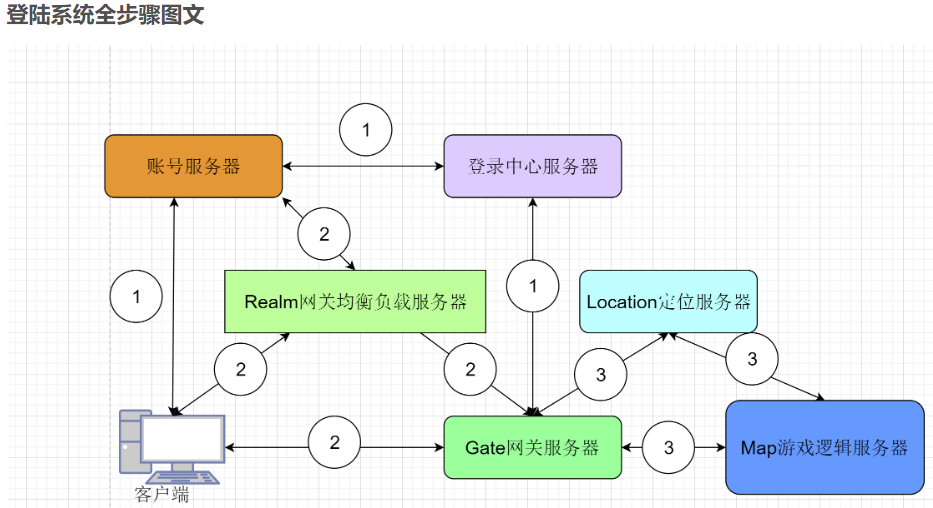
\includegraphics[width=.9\linewidth]{./pic/readme_20230124_102951.png}
\subsection{一. 账号登录}
\label{sec-3-1}
\subsubsection{1.客户端请求获取账户信息}
\label{sec-3-1-1}

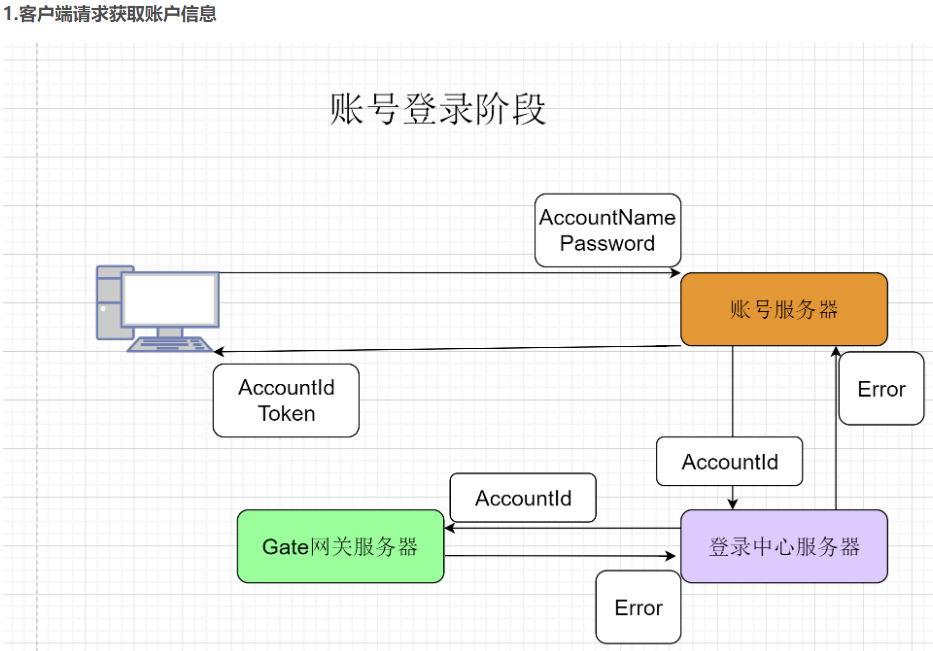
\includegraphics[width=.9\linewidth]{./pic/readme_20230124_103209.png}
\begin{itemize}
\item 客户端向账号服务器发送账户名和密码的消息,请求进行登录
\item 账号服务器和数据库交互,对信息进行验证或注册,获取账户唯一标识AccountId
\item 处理顶号逻辑,向登录中心服务器发送请求消息包含AccountId
\item 登录中心的组件存有AccountId和其所在区服zone的映射,若不存在AccountId直接返回即可
\item 若存在AccounId,根据其所在区服zone获取网关服务器的InstanceId,进而向其发送下线消息
\item 网关服务器存有所有客户端的映射实体Player(存有sessionInstanceId,UnitId,AccountId等)
\item 根据AccountId获取Player并通过Player的SessionInstanceId获取网关到客户端的session并释放
\item 为Player添加下线组件PlayerOfflineOutTimeComponent 后 返回即可
\item 登陆中心接到返回消息继续返回给账号服务器即可
\item 账号服务器处理完顶号逻辑后,自身也应缓存AccountId和自身的SessionId,做一次自身的顶号逻辑
\item 最后随机生成一个Token,把Token和AccountId发回给客户端
\item 客户端将AccountId Token等基本信息保存在zoneScene的AccountInfo组件中,供后续使用
\end{itemize}
\subsubsection{2. 客户端请求获取区服信息}
\label{sec-3-1-2}

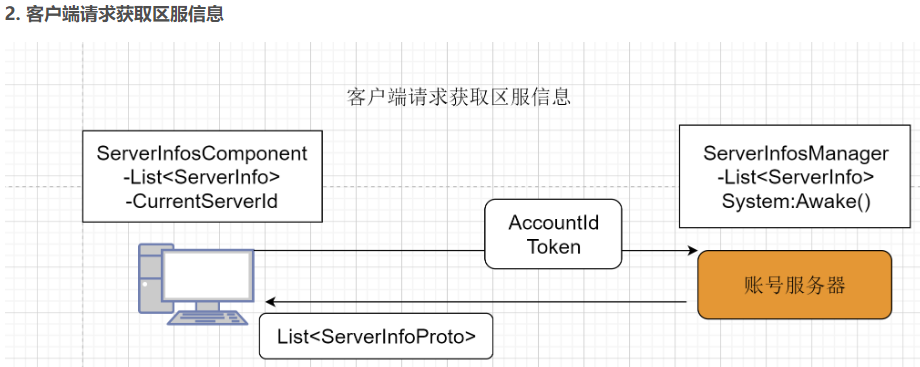
\includegraphics[width=.9\linewidth]{./pic/readme_20230124_103245.png}
\begin{itemize}
\item 定义ServerInfo区服信息实体(区服名,状态)及与proto映射的相互转换行为,并在双端均定义组件用以保存区服信息列表。
\item 服务器的组件要为其添加行为,Awake时就应该将数据库中的区服信息读取出来放入组件的信息列表中
\item 客户端向账号服务器发送信息,请求获取所有的区服信息,需要发送AccountId和Token用于验证账户
\item 账号服务器将服务器信息列表转换为其对应的ServerInfoProto列表,并发送回客户端
\item 客户端接收到后将proto转换回ServerInfo并保存到组件当中,显示到UI层供用户选择。
\item \textbf{注意 ServerInfoProto存在的意义,ET框架下网络传输的必须是Proto对象,不能直接是实体,所以需要定义Proto作为传输对象,在双端进行转换使用。}
\end{itemize}
\subsubsection{3. 客户端请求 获取/创建/删除 角色信息}
\label{sec-3-1-3}
\begin{enumerate}
\item 获取角色信息
\label{sec-3-1-3-1}

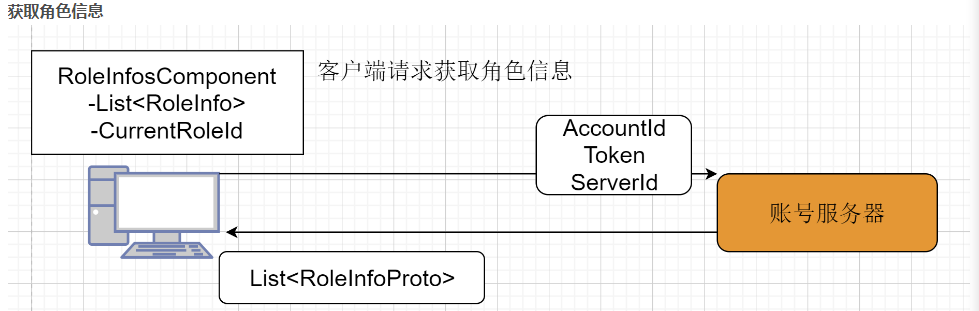
\includegraphics[width=.9\linewidth]{./pic/readme_20230124_103354.png}
\begin{itemize}
\item 获取角色信息的步骤和获取服务器信息很类似
\begin{itemize}
\item 定义RoleInfo实体(Name,AccountId,State,ServerId),并为其提供和proto的相互转换行为
\item 实体是双端可以公用的,但账号服务器无需保存,只需在请求时从数据库获取完发回即可
\item 客户端向服务器发送消息请求获取 当前账户在当前区服下的所有未冻结的角色
\item 服务器通过Id和Token验证身份后,从数据库中获取所有角色信息转换成proto对象发回客户端
\item 客户端收到后将proto转换成RoleInfo存储在相应的组件中,显示到UI层供用户选择。
\end{itemize}
\end{itemize}
\item 创建角色信息
\label{sec-3-1-3-2}

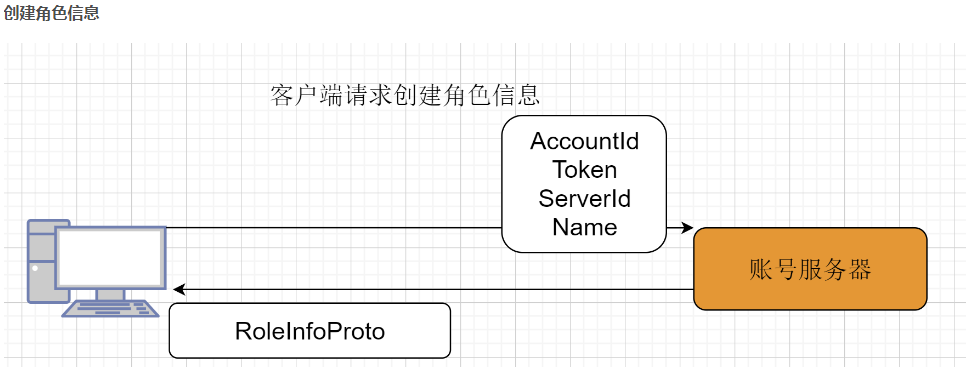
\includegraphics[width=.9\linewidth]{./pic/readme_20230124_103625.png}
\begin{itemize}
\item 用户和UI交互输入名称并点击按钮创建角色
\item 将用于验证的信息以及ServerId和用户输入的姓名一并发向服务器请求创建角色(区服间角色独立)
\item 服务器判断是否有重复角色,若没有则创建新角色RoleInfo,并对其各属性进行初始化。
\item 初始化利用Id创建使用GenerateUnitId,创建完成后保存到数据库中并转换成Proto发回客户端
\item 客户端收到RoleInfoProto后转换成RoleInfo并缓存起来,然后在UI管理处进行刷新UI循环列表
\end{itemize}
\item 删除角色信息
\label{sec-3-1-3-3}

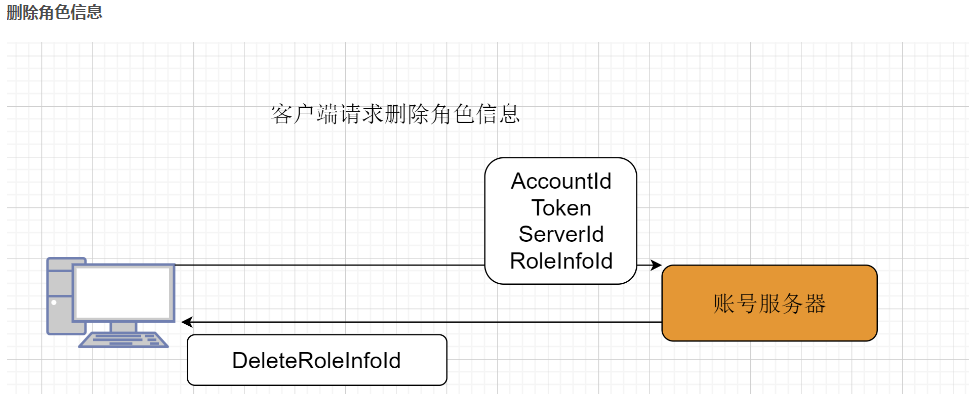
\includegraphics[width=.9\linewidth]{./pic/readme_20230124_103649.png}
\begin{itemize}
\item 在UI界面的循环列表为每个角色添加选择按钮,选择后会为组件的CurrentRoleId赋值选中的角色
\item 向账号服务器发送请求删除角色的信息,其中的RoleInfoId即为选择的CurrentRoleId。
\item 账号服务器在客户端中查询到指定Id的RoleInfo将其状态设置为Freeze冻结并修改名称(防止后续注册同名问题)
\item 发回客户端删除的RoleInfo的Id,客户端接收后在组件集合中将其移除并刷新UI界面。
\end{itemize}
\end{enumerate}
\subsection{二. 网关服务器的连接}
\label{sec-3-2}

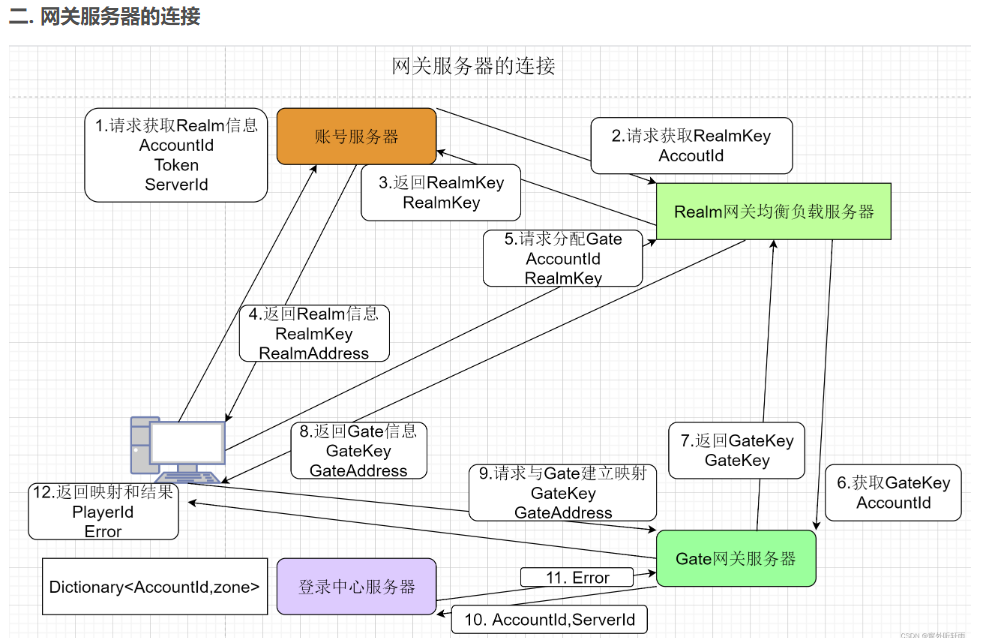
\includegraphics[width=.9\linewidth]{./pic/readme_20230124_103753.png}
\begin{itemize}
\item 网关服务器的的连接其实就是,客户端先和Realm网关连接请求其分配一个Gate网关,然后客户端去连接此Gate网关。
\end{itemize}
\subsubsection{1. 请求连接Realm网关}
\label{sec-3-2-1}
\begin{itemize}
\item 向账号服务器请求获取Realm网关的地址和令牌,需要区服Id,一般一个区服下有一个Realm
\item 账号服务器通过配置文件获取Realm网关的内网地址(sceneInstanceId),并向其请求获取RealmKey令牌。
\item Realm网关随机生成令牌RealmKey 和 AccountId将映射保存在组件中,将Key发回账号服务器
\item 账号服务器通过配置文件获取Realm网关的外网地址(OuterIPPort),和令牌RealmKey一并发回客户端
\end{itemize}
\subsubsection{2. 请求和Gate网关连接}
\label{sec-3-2-2}
\begin{itemize}
\item 客户端与账号服务器断连,与Realm建立连接,并向其请求分配网关服务器(即获取一个网关信息)
\item 一个区服下一般有多个Gate,Realm通过与账户Id取模的方式固定分配给此账户一个Gate,向此Gate请求获取GateKey
\item Gate网关服务器随机生成一个GateKey并将AccountId和GateKey的映射关系保存供后续验证,并发回Key
\item Realm服务器将Gate信息(key,address-配置文件得)发回客户端,客户端与Realm进行断开,准备连Gate
\end{itemize}
\subsubsection{3. 建立Gate映射对象Player}
\label{sec-3-2-3}
\begin{itemize}
\item 客户端一般会与Gate长时间连线,需要为Session添加心跳组件PingComponent,请求在Gate中创建映射对象Player
\item 步骤10 和 步骤11,主要是客户端与Gate建立连接后,将账户Id和区服号发送至登陆中心服务器进行注册添加,登录逻辑中会通过此服务器的记录进行顶号逻辑,通过区服号和AccountId利用Realm帮助类能唯一确定Gate,再给Gate发送下线消息即可。
\end{itemize}
\subsubsection{建立Player步骤}
\label{sec-3-2-4}
\begin{itemize}
\item 建立Player实体(AccountId,UnitId,SessionInstanceId,state),Player和账户ID,网关和客户端的Session连接以及Unit达到一一对应
\item 为网关到客户端的Session添加PlayerComponent保存所有Player实体(AccountId和Player映射字典),并为其添加SessionStateComponent,用于判断网关连接是否处于Normal或Game(便于后续Unit逻辑)
\item 为网关到客户端Session添加SessionPlayerComponent组件(AccountId,PlayerInstanceId)和Player一一对应,即在网关连接Session的此组件上直接获取相应Player,这样处理后续的游戏逻辑就不用每次都发送AccountId从PlayerComponent中获取了(节省传输量)
\item 判断是否可以复用Player,顶号下线时可以复用(后面有流程图解释),如果复用必须移除Player身上的下线组件,更新Session,即更新Player身上的SessionInstanceId和Session身上的SessionPlayerComponent重新创建。
\item 如果不是顶号等操作,直接创建Player并初始化即可,PlayerId用RoleId,UnitId暂时用RoleId,后续创建出游戏逻辑服Unit后用其替换。
\end{itemize}
将PlayerId返回给客户端供客户端可能使用。
\subsection{三. 游戏逻辑服务器连接}
\label{sec-3-3}
-​ 游戏逻辑服务器的连接本质上并不是客户端和其直接相连,而是通过在游戏服务器上建立一个映射对象和客户端绑定,客户端以后即可通过此映射对象的Id,通过网关转发和Location服务器的定位,将消息发送到服务器下的映射对象中。

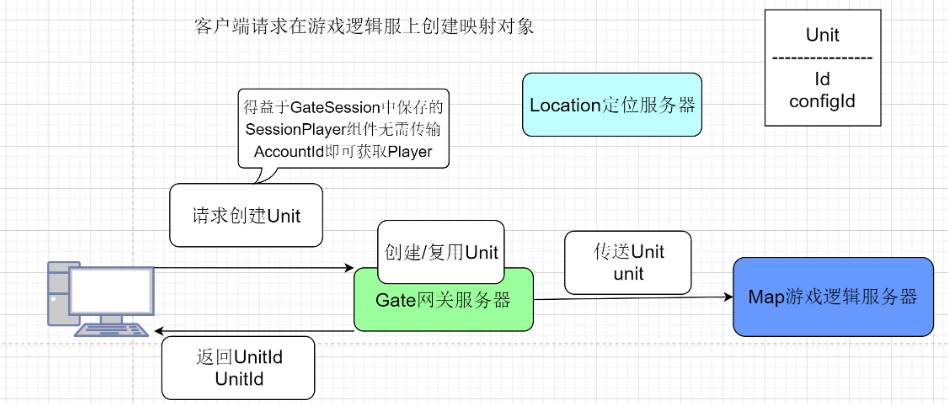
\includegraphics[width=.9\linewidth]{./pic/readme_20230124_103930.png}
\begin{itemize}
\item 客户端向Gate网关请求在Map服务器上创建Unit映射对象
\item 网关服务器先判断是否是顶号操作(利用Player的状态并向Player的Unit发送测试消息),验证成功后可以直接复用Player下的Unit并将UnitId返回客户端。
\item 若非顶号,则需要先临时为Player添加gateMapComponent组件,其下有一个属性Scene,在此Scene中创建一个Map场景用于后续传送Unit,(TransferHelper只能用于Map场景的传送,所以才做这一步)
\item 在上述创建的Map场景下创建Unit对象,UnitId可直接使用Player的Id即RoleId,然后必须为Unit添加UnitGateComponent,其中保存了gateSessionActorId即gateSessionInstanceId,(这样就可以利用Unit直接给客户端下发消息了)。
\item 利用配置文件获取Map服务器地址,利用TransferHelper的Transfer函数将unit传送到Map游戏逻辑服务器中
\item Transfer传送实现机制,实现以下机制后返回消息
\begin{itemize}
\item 通知客户端切换场景(直接利用unit下组件中gateSessionInstanceId直接下发即可)
\item request消息中保存Unit并将Unit下所有实现了ITransfer接口的组件保存起来一会一起传输过去
\item 删除当前Unit下的MailBoxComponent让发给此Unit的消息重发到正确位置(可能Unit还没传输过去就有信息发过来了)
\item 对Location定位服务器进行加锁,发送IActor消息传输给Map服务器,并释放当前Unit
\item Map服务器接收到消息将Unit和其组件重新添加(AddChild)到在此服务器下的UnitComponent中,将Unit添加到此组件集合中(传输时无法传输原Unit对象下的组件,只能将原Unit下基础属性以proto传递过来,在此还需重新生成)
\item 向客户端发相应的消息和属性,让客户端同步显示出角色并将Unit实体加入AOIEntity(AOI作用笔者暂且还未研究大概跟客户端有联系)
\end{itemize}
\item 传送完毕后将UnitId传回客户端即可,后续客户端就可利用UnitId发送IActorLocation消息和服务器上的Unit发送消息了。
\end{itemize}
\subsection{四. 顶号逻辑流程图}
\label{sec-3-4}

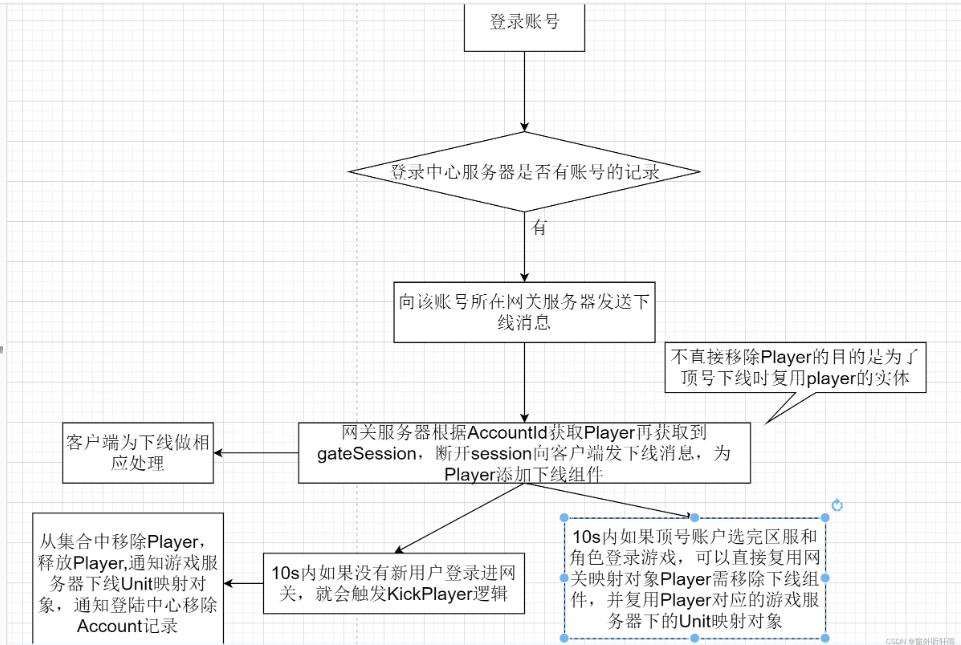
\includegraphics[width=.9\linewidth]{./pic/readme_20230124_104006.png}
\begin{itemize}
\item ​顶号逻辑属于是账号系统较为复杂的逻辑,其主要用到了中心登录服务器暂存玩家当前状态,并创建了Player和Unit映射对象,通过Player暂存到网关中实现顶号逻辑 可以无需重新创建Player和Unit直接更新属性复用,大大提高了顶号的效率。
\end{itemize}

\section{帐户服 + 数据库 + 登录中心服 + 网关服: 具体设计逻辑相关实现源码学习}
\label{sec-4}
\begin{itemize}
\item 上面是别人总结出来的大框架, 现在看仍是如云里雾里.项目是可以运行起来,并有demo小项目可以参考的
\item 可以根据上面的步骤与日志,把运行过程中的游戏端(ServerClient模式)游戏热更新Model.dll Hotfix.dll的源码看懂,弄明白这个框架是如何实现登录相关,以及必要的游戏逻辑服务器热更新的(如果有多余时间的话),应该就会对这个框架有相对更好的理解,可以考虑开始适配自己的简单服务器
\item 可以比较两种不同的启动模式有什么不同?
\item 先去找游戏客户端里,程序的入口是在哪里,逻辑如何连贯起来的? 因为项目比较大,看一次不曾自己真正实现过,狠容易就看一次忘记一次,所以记好笔记狠重要
\item MangoDB 数据库的连接,要把这个配置好,才能真正理解这个框架与范例
\end{itemize}

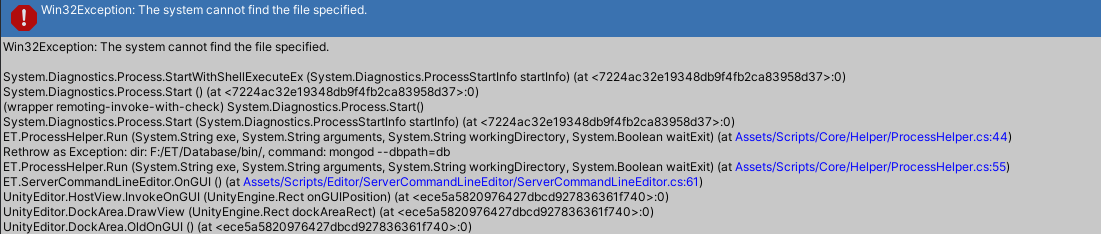
\includegraphics[width=.9\linewidth]{./pic/readme_20230124_111807.png}

\section{Bson 序列化与反序列化: Core/MongoHelper.cs 零碎的知识点大概总结在这些部分}
\label{sec-5}
\begin{itemize}
\item Mongo Bson非常完善,是我见过功能最全使用最强大的序列化库,有些功能十分贴心。其支持功能如下:
\begin{itemize}
\item 支持复杂的继承结构
\item 支持忽略某些字段序列化
\item 支持字段默认值
\item 结构多出多余的字段照样可以反序列化,这对多版本协议非常有用
\item 支持ISupportInitialize接口使用,这个在反序列化的时候简直就是神器
\item 支持文本json和二进制bson序列化
\item MongoDB数据库支持
\end{itemize}
\item 这里看一个关于反序列化时的继承关系所涉及到的点:
\item 支持复杂的继承结构
\item mongo bson库强大的地方在于完全支持序列化反序列化继承结构。需要注意的是, \textbf{继承反序列化需要注册所有的父类} ,有两种方法:
\item a. 你可以在父类上面使用[BsonKnownTypes]标签声明继承的子类,这样mongo会自动注册,例如:
\end{itemize}
\begin{minted}[fontsize=\scriptsize,linenos=false]{csharp}
    [BsonKnownTypes(typeof(Entity))]
    public class Component
    {
    }
    [BsonKnownTypes(typeof(Player))]
    public class Entity: Component
    {
    }
    public sealed class Player: Entity
    {
        public long Id;

        public string Account { get; set; }

        public long UnitId { get; set; }
    }
\end{minted}
\begin{itemize}
\item 这样有缺陷,因为框架并不知道一个类会有哪些子类, \textbf{这样做对框架代码有侵入性,我们希望能解除这个耦合 。}
\item b. 可以扫描程序集中所有子类父类的类型,将他们注册到mongo驱动中
\end{itemize}
\begin{minted}[fontsize=\scriptsize,linenos=false]{csharp}
Type[] types = typeof(Game).Assembly.GetTypes();
foreach (Type type in types)
{
    if (!type.IsSubclassOf(typeof(Component)))
    {
        continue;
    }

    BsonClassMap.LookupClassMap(type); // <<<<<<<<<<<<<<<<<<<< 
}
BsonSerializer.RegisterSerializer(new EnumSerializer<NumericType>(BsonType.String));
\end{minted}
\begin{itemize}
\item 这样完全的自动化注册,使用者也不需要关系类是否注册。
\item 这里还有点儿别的比较有价值的,但是今天没有看完:\url{https://www.kktoo.com/wiki/etnotes/chapter1/3.2\%E5\%BC\%BA\%E5\%A4\%A7\%E7\%9A\%84MongoBson\%E5\%BA\%93.html}  就是感觉要看ET框架中的源码,看正看明白了才会懂,现在看剩下的部分仍然是不懂(改天再看)
\end{itemize}
\section{后面消息处理的部分大致逻辑:《参考网上的:可对对照源码,把它不懂的也解惑了。。。》}
\label{sec-6}
\begin{itemize}
\item 在消息处理这方面,它的逻辑是这样的,
\item \url{https://blog.csdn.net/qq_33574890/article/details/128244264?spm=1001.2101.3001.6650.3&utm_medium=distribute.pc_relevant.none-task-blog-2\%7Edefault\%7EYuanLiJiHua\%7EPosition-3-128244264-blog-88990234.pc_relevant_aa2&depth_1-utm_source=distribute.pc_relevant.none-task-blog-2\%7Edefault\%7EYuanLiJiHua\%7EPosition-3-128244264-blog-88990234.pc_relevant_aa2&utm_relevant_index=4} 大家最开始也都同我一样,一知半解的,总有个熟悉的过程
\item\relax [与自己项目的本区别:] 自己的不是网络游戏,手游移动端,不是实现游戏模型逻辑的部分热更新,而是游戏的全部逻辑除了游戏入口在正常游戏程序域,其它都可以都全部放入了热更新程序域。所以自己的热更新并不涉及任何游戏过程逻辑与游戏逻辑服的交互,简化了无限多的大型网络游戏的逻辑模型热更新的步骤。下面ET框架更多的是用于大型网游的吧。。。。。
\item 在点击进入地图的按钮之后他会发送一个消息到服务器,服务器会发送一个玩家ID回来(这些都是,游戏过程中,一个客户端与游戏逻辑服的《实时?异步]交互)
\item 这个玩家ID就是客户端的唯一标识
\item 在收到服务器的回复消息时,再发送一个创建Unit的内部消息
\item 这个内部消息的处理者会创建这个Unit并进行广播,为什么要广播,不是很懂》[不是要适配大型多人网络游戏吗,不广播新的玩家进来了,其它玩家如何知晓呢]?为什么不用事件而要用内部消息也很奇怪《事件系统可以区分不同玩家吗?消息机制可以跨进程,可以这个玩家发给同区不同区其它玩家跟发短信一样,广播消息都都用actor消息机制吗?为什么要用事件系统,事件系统定义了玩家生成,玩家步移,玩家跳动跑动,玩家打架,玩家失血,玩家挂掉了吗?本质上讲应该似乎两种都可以,但消息机制可能更为简单广泛通用?》?
\item 在创建Unit的时候在他身上挂载了寻路组件和移动组件(如果是事件系统,就只有玩家生成,与玩家移动两个事件了吗?最主要的,事件系统是否定义了关于玩家这些逻辑的所有相关功能模块?没有,上面就是消息机制最为简单)。
\item 而游戏场景里面有一个OperaCompoent,这个组件会实时监听按键的点击并且将点击的位置发送给服务器,服务器再传送回客户端
\item 这边也挺奇怪的,[不奇怪,实现的是功能逻辑的元件组件化,可装载可卸载,相对更容易理解与精减维护源码]
\item 客户端这边接收ClickMapActor消息后解析位置,调用unit的Path组件进行移动。大体流程就是这样。
\item 但其实这样很不连贯,我发送一个消息,应该await等待获得消息,然后再做处理,这样就弄的 *很分散不够集中*[这个是说得很精准,以致于我现在入口加载都找上几十个文件弱弱拎不清楚。。。。。]
\end{itemize}

\section{事件处理}
\label{sec-7}
\begin{itemize}
\item ET的所有逻辑全部用事件来处理了
\item 这带来一个坏处,就是没办法高内聚。《为什么要高内聚呢?本来目的出发点就是要低内聚,减少功能模块逻辑的偶合decoupling呀》
\item 本来属于一个业务模型里面的逻辑,通过事件分散到了两到三个脚本里面。增加了阅读难度和上下连贯性。《这是如亲爱的表哥眼中的弱弱活宝妹般,小弱弱们读大型多人网络游戏框架的必经之痛,都得有这个过程》
\item 单纯举例来说,游戏初始化后发送了InitScenFinish事件。
\item UI处理模块接收到事件创建UI物体并显示
\item 在各个UI单独的组件比如LoginCom和LobbyCom里面进行UI逻辑撰写即并绑定事件
\item 他把本属于Model层的代码全部写进了静态类Helper里面来调用。《是这样吗???》
\item 也就是说View层直接调用了Model层代码。其实这样就强耦合了。《以小人之心度君子之腹,明明你自己也承认是帮助类,帮助类就不该是模型逻辑层?!在如亲爱的表哥眼中的活宝妹般弱弱的年代,这类错误概念设计上的理解,都是小弱弱们的辛酸泪,成长的代价。。。。。爱表哥,爱生活!!!》
\item 直接调用MapHelper
\item 上面就当从网络上搜来的梗概提要,等自己读源码的时候对照来理解,修正补确
\end{itemize}
\section{BuildModelAndHotfix: 一定要构建生成热更新程序集,项目狠大,两个程序集的内容没能消化好}
\label{sec-8}

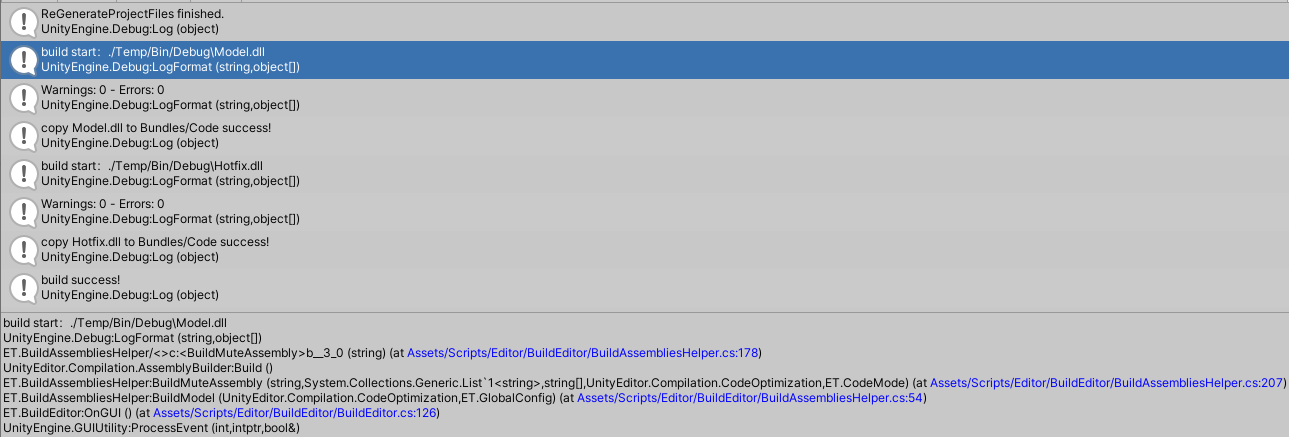
\includegraphics[width=.9\linewidth]{./pic/readme_20230125_103303.png}
\begin{itemize}
\item 它有几种不同的启动模式,可以再具体区分一下
\item 这里面有好多个项目,也要区分哪些是可以热更新,哪些是不能够热更新的,
\begin{itemize}
\item 没细看源码,竟然不知道, Unity.Model里面的代码不能热更新,通常将游戏中不会变动的部分放在这个项目里
\end{itemize}
\item 下面是根据范例加载过程的追踪来理解这么多个工程。自己项目的热更新等程序集都能弄懂并解决所有的问题。但是这个项目太大,感觉现在仍然有点儿无从下口的状态。。。。。
\end{itemize}
\section{Init.cs: 程序真正的入口}
\label{sec-9}
\begin{minted}[fontsize=\scriptsize,linenos=false]{csharp}
public class Init: MonoBehaviour {

    private void Start() {
        DontDestroyOnLoad(gameObject);
            
        AppDomain.CurrentDomain.UnhandledException += (sender, e) => {
            Log.Error(e.ExceptionObject.ToString());
        };
                
        Game.AddSingleton<MainThreadSynchronizationContext>(); // 线程上下文的无缝切换,可以高枕无忧不用管了
        // 命令行参数
        string[] args = "".Split(" ");
        Parser.Default.ParseArguments<Options>(args)
            .WithNotParsed(error => throw new Exception($"命令行格式错误! {error}"))
            .WithParsed(Game.AddSingleton);

// 注意,每个被Add的组件,都会执行其Awake(前提是他有类似的方法),这也是ETBook中的内容,不懂的同学回去补课哦
        Game.AddSingleton<TimeInfo>();
        Game.AddSingleton<Logger>().ILog = new UnityLogger();
        Game.AddSingleton<ObjectPool>();
        Game.AddSingleton<IdGenerater>();
        Game.AddSingleton<EventSystem>();
        Game.AddSingleton<TimerComponent>();
        Game.AddSingleton<CoroutineLockComponent>();
            
        ETTask.ExceptionHandler += Log.Error;
        Game.AddSingleton<CodeLoader>().Start(); // <<<<<<<<<<<<<<<<<<<< 
    }
        
// 框架中关注过的,几个统一管理的生命周期回调函数的一致系统化管理调用. 
    private void Update() {
        Game.Update(); // <<<<<<<<<< 
    }
    private void LateUpdate() {
        Game.LateUpdate(); // <<<<<<<<<< 
        Game.FrameFinishUpdate(); // <<<<<<<<<< 
    }
    private void OnApplicationQuit() {
        Game.Close(); // <<<<<<<<<< 
    }
}
\end{minted}
\section{Game.cs: 这个类会涉及到一些生命周期的管理等}
\label{sec-10}
\begin{minted}[fontsize=\scriptsize,linenos=false]{csharp}
public static class Game {
    [StaticField]
    private static readonly Dictionary<Type, ISingleton> singletonTypes = new Dictionary<Type, ISingleton>();
    [StaticField]
    private static readonly Stack<ISingleton> singletons = new Stack<ISingleton>();
    [StaticField]
    private static readonly Queue<ISingleton> updates = new Queue<ISingleton>();
    [StaticField]
    private static readonly Queue<ISingleton> lateUpdates = new Queue<ISingleton>();
    [StaticField]
    private static readonly Queue<ETTask> frameFinishTask = new Queue<ETTask>();

    public static T AddSingleton<T>() where T: Singleton<T>, new() {
        T singleton = new T();
        AddSingleton(singleton);
        return singleton;
    }

    public static void AddSingleton(ISingleton singleton) {
        Type singletonType = singleton.GetType();
        if (singletonTypes.ContainsKey(singletonType)) {
            throw new Exception($"already exist singleton: {singletonType.Name}");
        }
        singletonTypes.Add(singletonType, singleton);
        singletons.Push(singleton);

        singleton.Register();
        if (singleton is ISingletonAwake awake) {
            awake.Awake(); // 如果它实现过该接口,就会自动调用这个回调函数
        }

        if (singleton is ISingletonUpdate) {
            updates.Enqueue(singleton);
        }

        if (singleton is ISingletonLateUpdate) {
            lateUpdates.Enqueue(singleton);
        }
    }

// 这个类里,只有这个方法是,等待异步执行结果结束的,但是即便执行结束了,可能还没有设置结果,会晚些时候再设置结果
    public static async ETTask WaitFrameFinish() { 
        ETTask task = ETTask.Create(true); // 从池里抓一个新的出来用
        frameFinishTask.Enqueue(task);     // 入队
// <<<<<<<<<<<<<<<<<<<< 这里是,异步等待任务的执行吗?应该是 假如开启了池,await之后不能再操作ETTask,否则可能操作到再次从池中分配出来的ETTask,产生灾难性的后果
        await task; 
    }

    public static void Update() {
        int count = updates.Count;
        while (count-- > 0) {
            ISingleton singleton = updates.Dequeue();
            if (singleton.IsDisposed()) {
                continue;
            }
            if (singleton is not ISingletonUpdate update) {
                continue;
            }

            updates.Enqueue(singleton);
            try {
                update.Update();
            }
            catch (Exception e) {
                Log.Error(e);
            }
        }
    }
    public static void LateUpdate() {
        int count = lateUpdates.Count;
        while (count-- > 0) {
            ISingleton singleton = lateUpdates.Dequeue();

            if (singleton.IsDisposed()) {
                continue;
            }
            if (singleton is not ISingletonLateUpdate lateUpdate) {
                continue;
            }

            lateUpdates.Enqueue(singleton);
            try {
                lateUpdate.LateUpdate();
            }
            catch (Exception e) {
                Log.Error(e);
            }
        }
    }
    public static void FrameFinishUpdate() {
        while (frameFinishTask.Count > 0) {
// 为什么我会觉得这里它只是把ETTask从任务队列里取出来,并不曾真正执行过呢?它是在什么时候执行的,逻辑在哪里?前面那个异步方法调用的时候就已经开始执行了
            ETTask task = frameFinishTask.Dequeue(); 
            task.SetResult();
        }
    }
    public static void Close() {
        // 顺序反过来清理: 反过来清理才能真正清理得干净
        while (singletons.Count > 0) {
            ISingleton iSingleton = singletons.Pop();
            iSingleton.Destroy();
        }
        singletonTypes.Clear();
    }
}
\end{minted}
\section{CodeLoader.cs: 加载热更新等各种程序集}
\label{sec-11}
\begin{minted}[fontsize=\scriptsize,linenos=false]{csharp}
public class CodeLoader: Singleton<CodeLoader> {

    private Assembly model; // <<<<<<<<<< Model.dll, Hotfix.dll

    public void Start() {
        if (Define.EnableCodes) {
            GlobalConfig globalConfig = Resources.Load<GlobalConfig>("GlobalConfig");
            if (globalConfig.CodeMode != CodeMode.ClientServer) {
                throw new Exception("ENABLE_CODES mode must use ClientServer code mode!");
            }
            Assembly[] assemblies = AppDomain.CurrentDomain.GetAssemblies();
            Dictionary<string, Type> types = AssemblyHelper.GetAssemblyTypes(assemblies);
            EventSystem.Instance.Add(types);
            foreach (Assembly ass in assemblies) {
                string name = ass.GetName().Name;
                if (name == "Unity.Model.Codes") {
                    this.model = ass;
                }
            }
            IStaticMethod start = new StaticMethod(this.model, "ET.Entry", "Start"); // <<<<<<<<<< 调用热更新静态方法入口
            start.Run();
        } else {
            byte[] assBytes;
            byte[] pdbBytes;
            if (!Define.IsEditor) {
                Dictionary<string, UnityEngine.Object> dictionary = AssetsBundleHelper.LoadBundle("code.unity3d");
                assBytes = ((TextAsset)dictionary["Model.dll"]).bytes;
                pdbBytes = ((TextAsset)dictionary["Model.pdb"]).bytes;
                HybridCLRHelper.Load();
            } else {
                assBytes = File.ReadAllBytes(Path.Combine(Define.BuildOutputDir, "Model.dll"));
                pdbBytes = File.ReadAllBytes(Path.Combine(Define.BuildOutputDir, "Model.pdb"));
            }
            this.model = Assembly.Load(assBytes, pdbBytes);
            this.LoadHotfix();
            IStaticMethod start = new StaticMethod(this.model, "ET.Entry", "Start");
            start.Run();
        }
    }
    // 热重载调用该方法
    public void LoadHotfix() {
        byte[] assBytes;
        byte[] pdbBytes;
        if (!Define.IsEditor) {
            Dictionary<string, UnityEngine.Object> dictionary = AssetsBundleHelper.LoadBundle("code.unity3d");
            assBytes = ((TextAsset)dictionary["Hotfix.dll"]).bytes;
            pdbBytes = ((TextAsset)dictionary["Hotfix.pdb"]).bytes;
        } else {
            // 傻屌Unity在这里搞了个傻逼优化,认为同一个路径的dll,返回的程序集就一样。所以这里每次编译都要随机名字
            string[] logicFiles = Directory.GetFiles(Define.BuildOutputDir, "Hotfix_*.dll");
            if (logicFiles.Length != 1) {
                throw new Exception("Logic dll count != 1");
            }
            string logicName = Path.GetFileNameWithoutExtension(logicFiles[0]);
            assBytes = File.ReadAllBytes(Path.Combine(Define.BuildOutputDir, $"{logicName}.dll"));
            pdbBytes = File.ReadAllBytes(Path.Combine(Define.BuildOutputDir, $"{logicName}.pdb"));
        }
        Assembly hotfixAssembly = Assembly.Load(assBytes, pdbBytes);
        Dictionary<string, Type> types = AssemblyHelper.GetAssemblyTypes(typeof (Game).Assembly, typeof(Init).Assembly, this.model, hotfixAssembly);
        EventSystem.Instance.Add(types);
    }
}
\end{minted}
\section{Entry.cs: Assets/Scripts/Codes/Model/Share/Entry.cs 不是真正的入口}
\label{sec-12}
\begin{minted}[fontsize=\scriptsize,linenos=false]{csharp}
namespace ET {

    namespace EventType {
        public struct EntryEvent1 {
        }   
        
        public struct EntryEvent2 {
        } 
        
        public struct EntryEvent3 {
        } 
    }

// 这是程序的固定入口吗 ?  不是   
    public static class Entry {
        public static void Init() {
        }

        public static void Start() {
            StartAsync().Coroutine();
        }
// 相关的初始化:Bson, ProtoBuf, Game.NetServices, Root etc
        private static async ETTask StartAsync() {
            WinPeriod.Init(); // Windows平台 Timer Tick的时间精度设置
            
            MongoHelper.Init();   // MongoDB 数据库的初始化: 这里像是没作什么工程,但涉及类相关所有静态变量的初始化  
            ProtobufHelper.Init();// 同上: 这个没有太细看,改天用到可以补上
            
            Game.AddSingleton<NetServices>(); // 网络连接初始化: 还没有理解透彻
            Game.AddSingleton<Root>();        // 它说是,管理场景根节点的,没看
            await Game.AddSingleton<ConfigComponent>().LoadAsync(); // Config组件会扫描所有的有ConfigAttribute标签的配置,加载进来
            await EventSystem.Instance.PublishAsync(Root.Instance.Scene, new EventType.EntryEvent1());
            await EventSystem.Instance.PublishAsync(Root.Instance.Scene, new EventType.EntryEvent2());
            await EventSystem.Instance.PublishAsync(Root.Instance.Scene, new EventType.EntryEvent3());
        }
    }
}
\end{minted}
\section{Root.cs UI 的启动过程}
\label{sec-13}

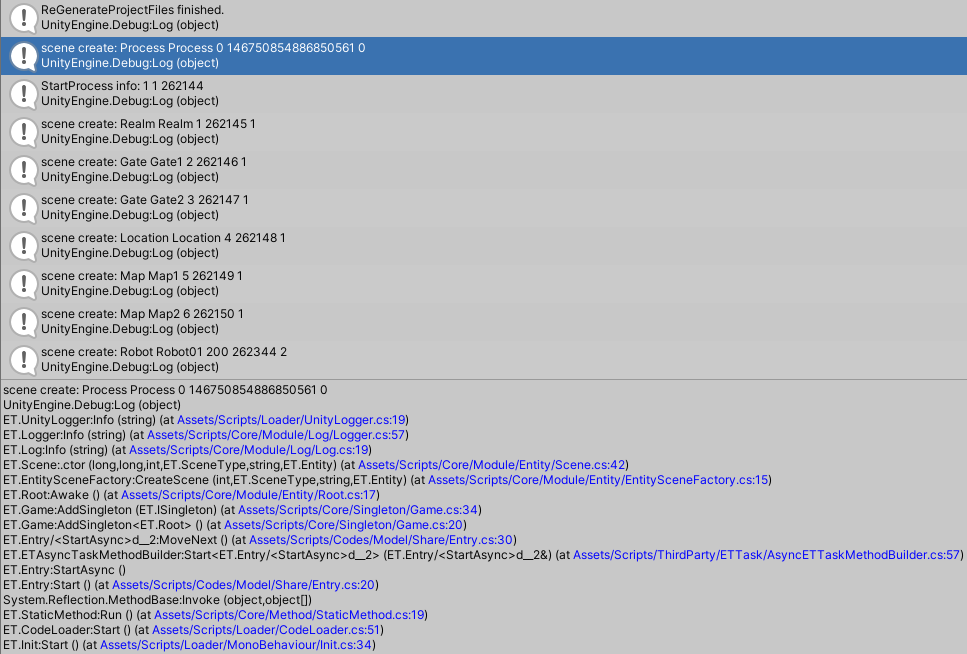
\includegraphics[width=.9\linewidth]{./pic/readme_20230125_092445.png}
\section{配置文件的加载过程:  就接上了ConfigComponent ?}
\label{sec-14}
\begin{itemize}
\item 在加载完服务端的Hotfix和Model的dll后,开始后面就是开始读取服务端的配置,并根据配置加载相应的组件。
\item 服务端的配置的读取方法使用的是CommandLine,该类用于读取命令行输入,并且将输入参数解析成Options类,存放在OptionComponent组件里面。[这里面的步骤还没有找]
\item 这里的参数来自客户端的配置文件,在Config$\backslash$StartConfig目录下。
\item 配置的读取是从客户端猫大写的工具里面读取的,具体在ServerCommandLineEditor类里面。
\end{itemize}
\section{ServerCommandLineEditor.cs:}
\label{sec-15}
\begin{minted}[fontsize=\scriptsize,linenos=false]{csharp}
  public enum DevelopMode {
      正式 = 0,
      开发 = 1,
      压测 = 2,
  }
  public class ServerCommandLineEditor: EditorWindow {
      [MenuItem("ET/ServerTools")]
      public static void ShowWindow() {
          GetWindow<ServerCommandLineEditor>(DockDefine.Types);
      }
      private int selectStartConfigIndex = 1;
      private string[] startConfigs;
      private string startConfig;
      private DevelopMode developMode;

      public void OnEnable() {
          DirectoryInfo directoryInfo = new DirectoryInfo("../Config/Excel/s/StartConfig");
          this.startConfigs = directoryInfo.GetDirectories().Select(x => x.Name).ToArray();
      }

      public void OnGUI() {
          selectStartConfigIndex = EditorGUILayout.Popup(selectStartConfigIndex, this.startConfigs);
          this.startConfig = this.startConfigs[this.selectStartConfigIndex];
          this.developMode = (DevelopMode) EditorGUILayout.EnumPopup("起服模式:", this.developMode);
          string dotnet = "dotnet.exe";
#if UNITY_EDITOR_OSX
          dotnet = "dotnet";
#endif
          if (GUILayout.Button("Start Server(Single Process)")) {
              string arguments = $"App.dll --Process=1 --StartConfig=StartConfig/{this.startConfig} --Console=1";
              ProcessHelper.Run(dotnet, arguments, "../Bin/");
          }
          if (GUILayout.Button("Start Watcher")) {
              string arguments = $"App.dll --AppType=Watcher --StartConfig=StartConfig/{this.startConfig} --Console=1";
              ProcessHelper.Run(dotnet, arguments, "../Bin/");
          }
          if (GUILayout.Button("Start Mongo")) {
              ProcessHelper.Run("mongod", @"--dbpath=db", "../Database/bin/");
          }
      }
  }
\end{minted}
\begin{itemize}
\item 感觉上面的配置类的定义,仍然是看得不明不白,看来这里得加把劲儿了
\item 启动服务器的时候,传递的参数如下:
\end{itemize}
\begin{minted}[fontsize=\scriptsize,linenos=false]{csharp}
string arguments = $"App.dll --appId={startConfig.AppId} --appType={startConfig.AppType} --config=../Config/StartConfig/{this.fileName}";
ProcessStartInfo info = new ProcessStartInfo("dotnet", arguments) { UseShellExecute = true, WorkingDirectory = @"../Bin/" };
\end{minted}
\begin{itemize}
\item 读取完配置后,将配置保存在StartConfigComponent组件里面,该组件在初始化时会根据配置的情况,分门别类将配置内容存进行缓存。接下来就是添加网络相关的组件OpcodeTypeComponent和MessageDispatherComponent组件,具体可看这篇文章《ET框架学习——OpcodeTypeComponent组件和MessageDispatherComponent组件》。\url{https://blog.csdn.net/Tong1993222/article/details/86600357}
\item 最后就是根据配置的AppType类型,添加对应的组件,这里我选择的是AllServer类型,所有相关组件都会添加,具体可以参看源码。
\item 当前链接: \url{https://blog.csdn.net/Tong1993222/article/details/88990234}
\item 下面是自己的理解: 程序最开始加载程序集的时候,或是某个什么地方(没能理解透彻),会自动扫描程序集中的带配置标签的配置,进行配置
\end{itemize}
\section{ConfigComponent.cs: Config组件会扫描所有的有ConfigAttribute标签的配置,加载进来}
\label{sec-16}
\begin{minted}[fontsize=\scriptsize,linenos=false]{csharp}
// Config组件会扫描所有的有ConfigAttribute标签的配置,加载进来
public class ConfigComponent: Singleton<ConfigComponent> {

    public struct GetAllConfigBytes {
    }
    public struct GetOneConfigBytes {
        public string ConfigName;
    }
    private readonly Dictionary<Type, ISingleton> allConfig = new Dictionary<Type, ISingleton>();

    public override void Dispose() {
        foreach (var kv in this.allConfig) {
            kv.Value.Destroy();
        }
    }
    public object LoadOneConfig(Type configType) {
        this.allConfig.TryGetValue(configType, out ISingleton oneConfig);
        if (oneConfig != null) {
            oneConfig.Destroy();
        }
        byte[] oneConfigBytes = EventSystem.Instance.Invoke<GetOneConfigBytes, byte[]>(0, new GetOneConfigBytes() {ConfigName = configType.FullName});
        object category = SerializeHelper.Deserialize(configType, oneConfigBytes, 0, oneConfigBytes.Length);
        ISingleton singleton = category as ISingleton;
        singleton.Register();
            
        this.allConfig[configType] = singleton;
        return category;
    }
        
    public void Load() {
        this.allConfig.Clear();
        Dictionary<Type, byte[]> configBytes = EventSystem.Instance.Invoke<GetAllConfigBytes, Dictionary<Type, byte[]>>(0, new GetAllConfigBytes());
        foreach (Type type in configBytes.Keys) {
            byte[] oneConfigBytes = configBytes[type];
            this.LoadOneInThread(type, oneConfigBytes);
        }
    }
        
    public async ETTask LoadAsync() {
        this.allConfig.Clear();
        Dictionary<Type, byte[]> configBytes = EventSystem.Instance.Invoke<GetAllConfigBytes, Dictionary<Type, byte[]>>(0, new GetAllConfigBytes());
        using ListComponent<Task> listTasks = ListComponent<Task>.Create();
            
        foreach (Type type in configBytes.Keys) {
            byte[] oneConfigBytes = configBytes[type];
            Task task = Task.Run(() => LoadOneInThread(type, oneConfigBytes)); // <<<<<<<<<<<<<<<<<<<< 
            listTasks.Add(task);
        }
        await Task.WhenAll(listTasks.ToArray());
        foreach (ISingleton category in this.allConfig.Values) {
            category.Register();
        }
    }
        
    private void LoadOneInThread(Type configType, byte[] oneConfigBytes) {
        object category = SerializeHelper.Deserialize(configType, oneConfigBytes, 0, oneConfigBytes.Length); // <<<<<<<<<<<<<<<<<<<< 
        lock (this) {
            this.allConfig[configType] = category as ISingleton;    
        }
    }
}
\end{minted}
\section{ConfigAttribute.cs: 就是空定义,用来标注这个标签就可以了}
\label{sec-17}
\begin{minted}[fontsize=\scriptsize,linenos=false]{csharp}
[AttributeUsage(AttributeTargets.Class)]
public class ConfigAttribute: BaseAttribute {
}
\end{minted}
\begin{itemize}
\item 上面的不是是扫描配置标签吗,扫描完了就根据配置标签来配置呀
\end{itemize}
\section{StartProcessConfig: ProtoObject, IConfig}
\label{sec-18}
\begin{itemize}
\item 这些自动生成的文件,还没有搞明白:为什么它们是自动生成的?为什么要把配置的过程定义成自动生成?一类配置自动生成的方法定义,在这个框架中有什么好处?可以提精提纯简化这类标签配置的源码吗?
\begin{minted}[fontsize=\scriptsize,linenos=false]{csharp}
  [ProtoContract]
[Config]
public partial class StartProcessConfigCategory : ConfigSingleton<StartProcessConfigCategory>, IMerge {
    [ProtoIgnore]
    [BsonIgnore]
    private Dictionary<int, StartProcessConfig> dict = new Dictionary<int, StartProcessConfig>();

    [BsonElement]
    [ProtoMember(1)]
    private List<StartProcessConfig> list = new List<StartProcessConfig>();

    public void Merge(object o) {
        StartProcessConfigCategory s = o as StartProcessConfigCategory;
        this.list.AddRange(s.list);
    }

    [ProtoAfterDeserialization]        
    public void ProtoEndInit() {
        foreach (StartProcessConfig config in list) {
            config.AfterEndInit();
            this.dict.Add(config.Id, config);
        }
        this.list.Clear();

        this.AfterEndInit();
    }

    public StartProcessConfig Get(int id) {
        this.dict.TryGetValue(id, out StartProcessConfig item);
        if (item == null) {
            throw new Exception($"配置找不到,配置表名: {nameof (StartProcessConfig)},配置id: {id}");
        }
        return item;
    }

    public bool Contain(int id) {
        return this.dict.ContainsKey(id);
    }
    public Dictionary<int, StartProcessConfig> GetAll() {
        return this.dict;
    }
    public StartProcessConfig GetOne() {
        if (this.dict == null || this.dict.Count <= 0) {
            return null;
        }
        return this.dict.Values.GetEnumerator().Current;
    }
}

[ProtoContract]
public partial class StartProcessConfig: ProtoObject, IConfig {
    // <summary>Id</summary>
    [ProtoMember(1)]
    public int Id { get; set; }
    // <summary>所属机器</summary>
    [ProtoMember(2)]
    public int MachineId { get; set; }
    // <summary>内网端口</summary>
    [ProtoMember(3)]
    public int InnerPort { get; set; }
}
\end{minted}
\end{itemize}
\section{partial class StartProcessConfigCategory : ConfigSingleton<StartProcessConfigCategory>, IMerge}
\label{sec-19}
\begin{minted}[fontsize=\scriptsize,linenos=false]{csharp}
[ProtoContract]
[Config]
public partial class StartProcessConfigCategory : ConfigSingleton<StartProcessConfigCategory>, IMerge {
    [ProtoIgnore]
    [BsonIgnore]
    private Dictionary<int, StartProcessConfig> dict = new Dictionary<int, StartProcessConfig>();

    [BsonElement]
    [ProtoMember(1)]
    private List<StartProcessConfig> list = new List<StartProcessConfig>();

    public void Merge(object o) {
        StartProcessConfigCategory s = o as StartProcessConfigCategory;
        this.list.AddRange(s.list);
    }

    [ProtoAfterDeserialization] // 它说这里就是提供的狠好用的接口,方便在反序列化之后进行什么必要的操作       
    public void ProtoEndInit() {
        foreach (StartProcessConfig config in list) {
            config.AfterEndInit(); // <<<<<<<<<<<<<<<<<<<< 
            this.dict.Add(config.Id, config);
        }
        this.list.Clear();

        this.AfterEndInit();
    }

    public StartProcessConfig Get(int id) {
        this.dict.TryGetValue(id, out StartProcessConfig item);
        if (item == null) {
            throw new Exception($"配置找不到,配置表名: {nameof (StartProcessConfig)},配置id: {id}");
        }
        return item;
    }

    public bool Contain(int id) {
        return this.dict.ContainsKey(id);
    }
    public Dictionary<int, StartProcessConfig> GetAll() {
        return this.dict;
    }
    public StartProcessConfig GetOne() {
        if (this.dict == null || this.dict.Count <= 0) {
            return null;
        }
        return this.dict.Values.GetEnumerator().Current;
    }
}
\end{minted}
\section{StartProcessConfig.cs:}
\label{sec-20}
\begin{minted}[fontsize=\scriptsize,linenos=false]{csharp}
public partial class StartProcessConfig {

    private IPEndPoint innerIPPort;
    public long SceneId;

    public IPEndPoint InnerIPPort {
        get {
            if (this.innerIPPort == null) {
                this.innerIPPort = NetworkHelper.ToIPEndPoint($"{this.InnerIP}:{this.InnerPort}");
            }
            return this.innerIPPort;
        }
    }

    public string InnerIP => this.StartMachineConfig.InnerIP;
    public string OuterIP => this.StartMachineConfig.OuterIP;
    public StartMachineConfig StartMachineConfig => StartMachineConfigCategory.Instance.Get(this.MachineId);

    public override void AfterEndInit() {
        InstanceIdStruct instanceIdStruct = new InstanceIdStruct((int)this.Id, 0);
        this.SceneId = instanceIdStruct.ToLong();
        Log.Info($"StartProcess info: {this.MachineId} {this.Id} {this.SceneId}");
    }
}
\end{minted}
\begin{itemize}
\item 不知道今天上午用VSC出什么问题,程序跑不通了,等再关几个窗口,重新运行得通的时候才可以再追踪日志,先等等
\item 它有几个模式:好像要有一个一一对应,就是一个服务器,一个客户端,大致的意思是说,同在游戏引擎里,不能一次弄出两三个客户端之类的吧(就是要么clientserver模式,要么server + client, 别弄了个servier,结果又构建了个clientserver)这样程序就可以正常运行了
\item 感觉那么追日志看得好艰难,跟不上.就先把游戏中需要打包构建的几个主要的程序自己先理解一遍,不懂的上网查,再跟着日志看。现在看感觉仍然不知道在哪里
\end{itemize}
\section{HotfixView程序域: 先看这部分,这里面的大部分的源码都还比较简单}
\label{sec-21}
\begin{itemize}
\item 应快把样例工程中的源码爬一遍
\item 现在基本的原理能够懂得: 把大的版块基本能够看得懂的地方看懂,也稍微总结一下.不懂的地方就用安卓应用快速地整几个应用来测试掌握一下
\item \textbf{Awake, Load, Update, LateUpdate, Destroy:} 这个系统最简单,无处不在,类似Unity3d的组件,ET框架也提供了组件事件,例如Awake,Start,Update等。要给一个Component或者Entity加上这些事件,必须写一个辅助类。
\item ET中大致类等的特点总结:
\begin{itemize}
\item Entity:对应一个真实物体(至少也是一个逻辑实体)。特征:一定有一个代表这个实体的唯一Id。
\item Component:一个实体针对某个特定片面的状态数据,比如位置数据。注意,要求只有数据不能有函数(基本的get,set类函数可以包含)
\item System:对Entity中某些Component进行计算和更改的方法集合
\item Utility函数:如果System之间相互依赖某些函数,则需要把这些函数提取为工具函数。也就是说,所有System之间需要确保不要太多相互依赖。
\item 单例Component:如果某个状态是全局的,而不是和某个具体实体相关的,则需要提取
\end{itemize}
\end{itemize}

\section{消息机制的原理,类图,总体概念理解}
\label{sec-22}
\begin{itemize}
\item \url{https://www.jianshu.com/p/f2ecf148bc2f}
\end{itemize}
\subsection{消息分类}
\label{sec-22-1}

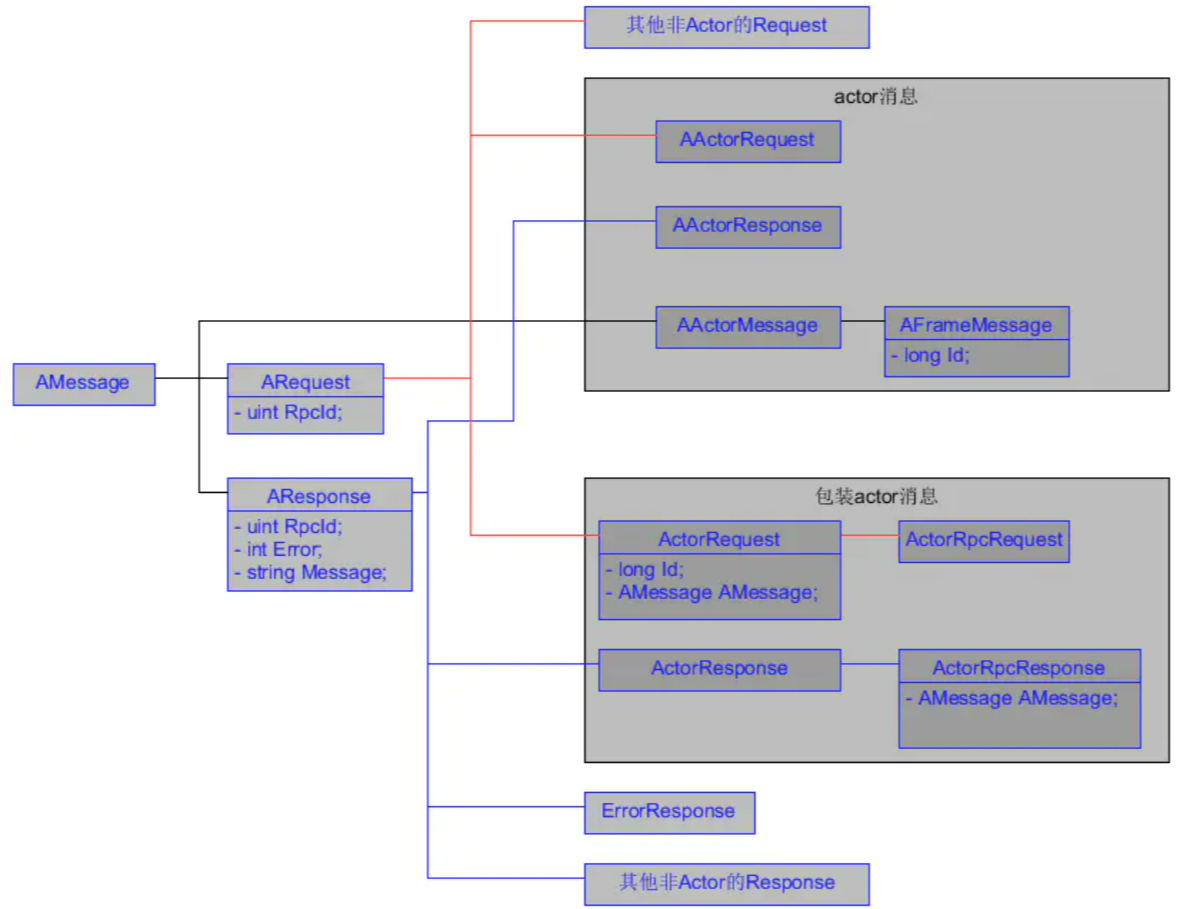
\includegraphics[width=.9\linewidth]{./pic/readme_20230127_113555.png}
\begin{itemize}
\item 消息按照因果关系分类,可以分为Request和Response,当然也有直接继承至Message的,表示我这个消息发出去后我就不care了。Request和Response是成对的,我发了一个Request,你必须回我一个对应的Response消息。
\item 消息还可以按照类型分类,基本分为两大类,一般消息和Actor消息。Actor消息可以认为是战斗相关消息,战斗unit和玩家client之间发送的都是Actor消息,比如帧同步消息(AFrameMessage)就是一种ActorMessage,其他的都可以认为是一般消息,比如登陆,创角等。
\item Actor相关的消息在服务器间相互转发的时候,会被包装一下。想象一下,一个Client与GateServer之间的通信,消息里面是不用带玩家角色Id的,我们之间的Session对象就表明了我的身份。但是GateServe把这个消息转发给MapServer的时候,消息就得包装一下,带上UnitId的信息,这样MapServer收到这个消息后才知道是那个玩家发过来的。包装actor消息包括ActorRequest和ActorRPCRequest,AActorMessage不需要回复,就包装在ActorRequest中,而AActorRequest需要回复,包装在ActorRPCRequest中。所以ActorRequest和ActorRPCRequest包括他们的回复消息只在服务器之间传送Actor消息的时候用。
\item 其实按照消息的路径,还可以把消息分为内部消息和外部消息,内部就是服务器内部之间发送的,外部则是负责服务器和客户端通信的。在ET中,有InnerMessage和OuterMessage两个文件,里面定义的消息就分别是内部和外部消息。只有Realm服务器和Gate服务器有NetOuterComponent,可以与客户端通信,其他服务器都只有NetInnerComponent,Realm服务器作为初始登陆服务器,负责分配Gate服务器给玩家,之后玩家都直接与Gate服务器通信,之后其他服务器都通过Gate服务器与玩家通信。
\end{itemize}

\subsection{ET 消息流程}
\label{sec-22-2}

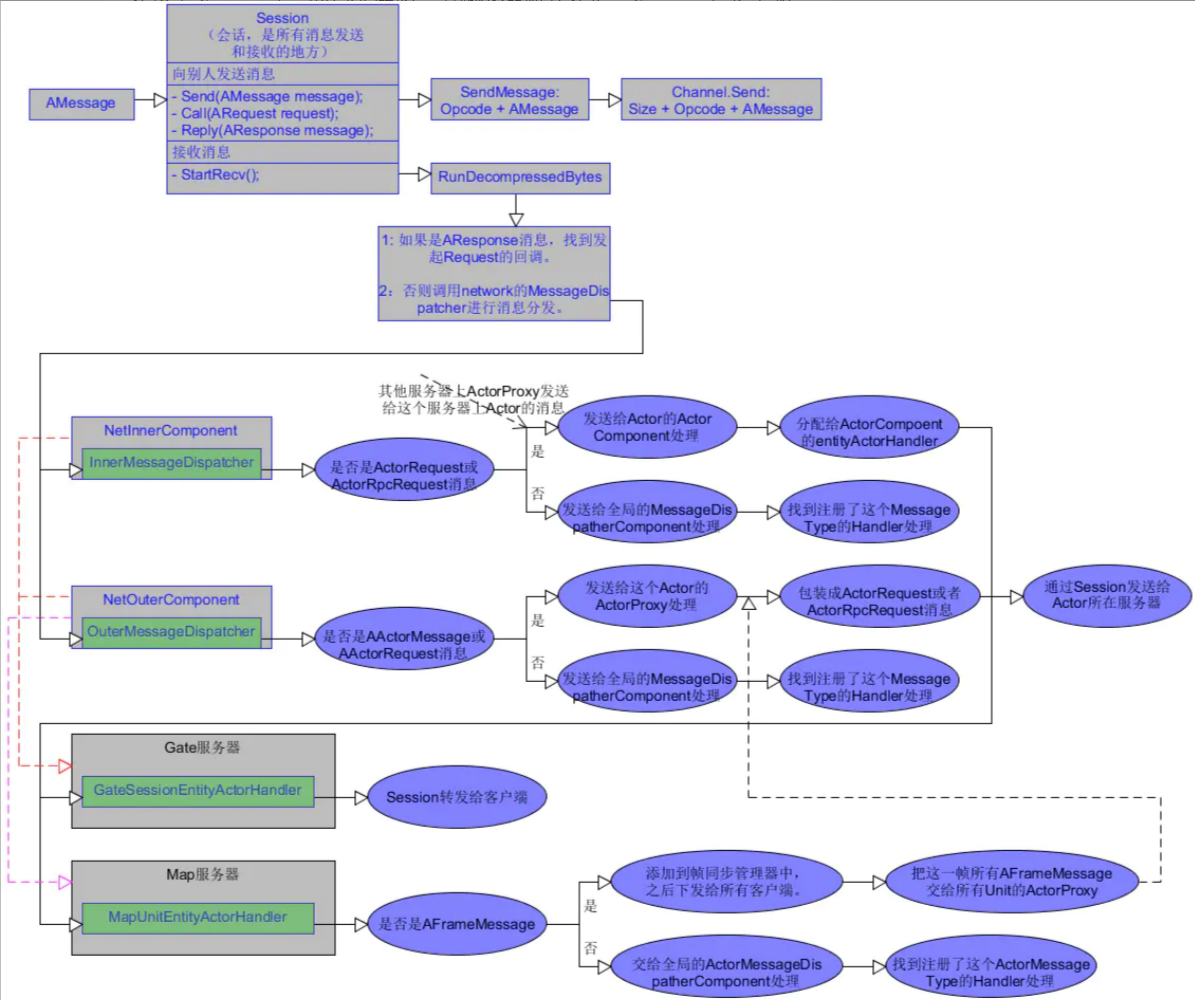
\includegraphics[width=.9\linewidth]{./pic/readme_20230127_113503.png}
\begin{itemize}
\item 这里面弄清了几个原则,基本就清楚了消息的处理原则:
\item 1:Gate服务器既需要与客户端通信,也需要与其他服务器通信。所以需要同时拥有NetOuterComponent和NetInnerComponent。
\item 2:Map服务器不直接与客户端通信,需要通过Gate服务器转发,所以只有NetInnerComponent。
\item 3:客户端发送给Gate服务器的消息,都是通过NetOuterComponent走的,所以Actor消息都是AActorMessage或者AActorRequest类型(因为Gate服务器上接收消息的Session就表明了客户端的身份),而这些Actor消息是需要转发给Map服务器的,Gate服务器和每个Map服务器之间都只有一个Session(属于NetInnerComponent),所有Actor消息都通过这个Session发送,所以Actor消息在这里需要包装成ActorRequest或者ActorRpcRequest消息,带actorId,Map服务器接收到这个消息后通过actorId才知道交给哪个Actor处理。
\item 4:Map服务器发送给Gate服务器的ActorRequest或者ActorRpcRequest消息,Gate服务器只需要把包装里面的AMessage发送给对应的客户端即可。
\item 这里加个链接:latex graphcs .9倍的图片宽度,修改的话可以尝试:\url{https://tex.stackexchange.com/questions/439918/set-default-value-for-max-width-of-includegraphics}
\end{itemize}
\subsection{这里,我在讲一下我自己的理解,方便看完后还是一脸懵逼的同学理解。}
\label{sec-22-3}
\begin{itemize}
\item 我们先别管那些类,我们先想想,我们需要发送的消息,都是些什么?
\begin{itemize}
\item 1. 客户端发送给服务器的消息
\item 1. 不需要与其他服务器通信(普通消息)
\item 1. 不需要返回结果(普通的普通消息)
\item 2. 需要返回结果(普通的RPC消息)
\item 2. 需要与其他服务通信(Actor消息)
\item 1. 不需要返回结果(普通的Actor消息)
\item 2. 需要返回结果(Actor RPC消息)
\item 2. 服务器发送给客户端的消息
\item 1. 返回客户端请求的消息(根据客户端的请求消息类型发送对应的回复类型)
\item 2. 主动发送的消息,比如帧同步消息。
\end{itemize}
\item 以上的属于服务端与客户端之间的消息类型,皆属于OuterMessage。(外部消息)
\item 3. 服务器与其他服务器对话的消息(属于内部消息InnerMessage,且是Actor消息)
\begin{itemize}
\item 1. 需要返回结果(Actor RPC消息)
\item 2. 不需要返回结果(普通的Actor消息)
\end{itemize}
\item 这里大家可以想象一下,服务器接收到其他服务器传来的Actor消息,其实就像是收到客户端传来的普通消息一样。所以InnerMessageDispatcher就没有必要再把消息发送给其他服务器上处理。
\item 简单的说,就是这样。
\begin{itemize}
\item 普通消息只要发送给一个服务器就能得到结果
\item actor消息可能得通过其他服务器才能得到结果
\item actor消息又分actor rpc消息,rpc消息会返回结果。
\end{itemize}
\end{itemize}
% Emacs 27.2 (Org mode 8.2.7c)
\end{document}